\section{Additional Grounding Results and Decoding Variability}
\label{app:archive}

The clean two-view task tests query binding; the larger archive exposes
behavior across repeated views and output conventions. Table~\ref{tab:archive}
compares six configurations using normalized two-line output. Its 30-pair
columns are exact-ID slices of the 80-pair inference runs, using the same saved
responses and current image digests. The 80-pair set includes repeated views
of 16 targets.

\begin{table}[htbp]
\centering\small
\setlength{\tabcolsep}{3pt}
% Generated by scripts/build_assets.py from corrected results.json
\begin{tabular}{lrrrrrr}
\toprule
Model & \multicolumn{2}{c}{Close views (30)} & \multicolumn{2}{c}{Mixed views (80)} & $\Delta$ (pp) & Flips \\
\midrule
Gemma4-E4B & 90.0 & 96.7 & 70.0 & 65.0 & -5.0 & 12/80 \\
Qwen2.5-VL-7B & 10.0 & 13.3 & 3.8 & 5.0 & +1.2 & 5/80 \\
Qwen3-VL-2B & 86.7 & 86.7 & 53.8 & 50.0 & -3.8 & 13/80 \\
Qwen3-VL-8B & 93.3 & 96.7 & 86.2 & 85.0 & -1.2 & 7/80 \\
InternVL3-8B & 60.0 & 66.7 & 35.0 & 40.0 & +5.0 & 16/80 \\
Molmo-7B-D & 90.0 & 96.7 & 92.5 & 93.8 & +1.2 & 5/80 \\
\bottomrule
\end{tabular}

\caption{Archived raster readout: end-to-end point hits (\%). Each pair of
columns reports Original then Converted. Differences and flips use all 80
pairs; all queries remain in the denominator.}
\label{tab:archive}
\end{table}

The close views and mixed views give different pictures of performance.
Gemma4 reaches 90.0/96.7\% on close views but 70.0/65.0\% over all 80 pairs.
InternVL3 gains five percentage points in the larger set while changing hit
status on 16 pairs. Qwen3-VL-2B changes status on 13 pairs despite a net decrease
of three hits. The larger archive thus reinforces the distinction between the
number of hits and the set of views on which those hits occur.

\subsection{The earlier clean pool and development probes}
Table~\ref{tab:app-clean15} reports the 15-pair pool spanning nine targets.
This pool precedes the repaired four-source construction. Gemma4 changes from
8 to 6 hits, Qwen3-VL-8B from 12 to 13, and Qwen2.5-VL records no hits under
the normalized frame. These outcomes remain tied to their saved inputs.

\begin{table}[htbp]
\centering\small
% Generated by appendix/build_tables.py; source hashes in table_sources.json.
\begin{tabular}{lrrrrrr}
\toprule
Model & $N$ & $V_O$ & $V_C$ & $H_O$ & $H_C$ & Flips \\
\midrule
Gemma4-E4B & 15 & 15 & 15 & 8 & 6 & 4 \\
InternVL3-8B & 15 & 13 & 11 & 3 & 3 & 2 \\
Qwen2.5-VL-7B & 15 & 14 & 15 & 0 & 0 & 0 \\
Qwen3-VL-2B & 15 & 15 & 15 & 3 & 3 & 2 \\
Qwen3-VL-8B & 15 & 15 & 15 & 12 & 13 & 1 \\
\bottomrule
\end{tabular}

\caption{The 15-pair grounding pool under normalized two-line readout.
$V$ counts numeric outputs and $H$ counts hits, both over $N=15$ per condition.
Flips count paired changes in hit status.}
\label{tab:app-clean15}
\end{table}

The four-pair pilot and 14-pair zoom study capture the development of the
readout protocol (Table~\ref{tab:app-historical}). The Gemma4 pilot requested
pixels but its normalized reinterpretation yields four original and three
converted hits. Qwen2.5's early JSON responses contain no parseable points;
the two-line prompt produces points but still exposes a scale mismatch.
In the zoom study, Gemma4 yields 11 and 13 normalized hits, while Qwen2.5 yields
three in each condition. Its pixel reinterpretation instead gives nine and
six. Recomputing these rows over every query preserves format failures in the
same denominator as localization failures.

\begin{table}[htbp]
\centering\small
\setlength{\tabcolsep}{4pt}
% Generated by appendix/build_tables.py; source hashes in table_sources.json.
\begin{tabular}{lrrrr}
\toprule
Run & $N$ & $V_O/V_C$ & Requested hits O/C & Other frame O/C \\
\midrule
Gemma4 pilot & 4 & 4/4 & 0/0 & 4/3 \\
Qwen2.5 JSON pilot & 4 & 0/0 & 0/0 & 0/0 \\
Qwen2.5 text pilot & 4 & 3/4 & 0/0 & 2/2 \\
Gemma4 zoom & 14 & 14/14 & 11/13 & 1/1 \\
Qwen2.5 zoom & 14 & 14/13 & 3/3 & 9/6 \\
\bottomrule
\end{tabular}

\caption{Earlier pilot and zoom runs, rescored from saved predictions with
fixed denominators. Entries separated by a slash are Original/Converted
counts. The Gemma4 pilot requested pixels; all other rows requested normalized
0--1000. ``Other frame'' applies the alternative interpretation uniformly.}
\label{tab:app-historical}
\end{table}

\subsection{Reading individual responses}
The recorded responses include several distinct cases:
a Gemma4 faucet point changes from a normalized hit to a miss while the answer
remains ``faucet''; Qwen2.5 returns a truncated ``fauc'' in a faucet example;
and a clock response changes from a pixel-frame miss to a hit. The examples
separate point movement, truncated answers, and coordinate interpretation.
Some archived inputs contain MDL compilation failures; their scores therefore
reflect rendering faults as well as material differences.
Figures~\ref{fig:app-diagnostic1} and~\ref{fig:app-diagnostic2} show matched
qualitative rerenders after MDL dependency repair. Historical predictions and
scores remain tied to their original inputs and are not transferred to these
new images.

\subsection{Stochastic spatial readout}
Three runs at temperature 0.7 evaluate each of the 60 images in the 30-pair
archive. Seed distance is the mean of the three pairwise pixel distances on
one image; hit status is variable when the three binary outcomes differ.
All queries in each model group have three numeric points.

\begin{table}[htbp]
\centering\small
% Generated by scripts/build_assets.py from corrected results.json
\begin{tabular}{lrrr}
\toprule
Model & Complete triples & Seed distance (px) & Hit variability (\%) \\
\midrule
Qwen3-VL-8B & 60/60 & 7.66 & 0.0 \\
Qwen3-VL-2B & 60/60 & 24.34 & 16.7 \\
Gemma4-E4B & 60/60 & 27.07 & 10.0 \\
\bottomrule
\end{tabular}

\caption{Stochastic readout on identical images. Complete triples count
queries with three numeric points. Seed distance is measured in image pixels;
hit-status variability counts queries whose three outcomes differ.}
\label{tab:sampling}
\end{table}

Qwen3-VL-8B combines the smallest mean seed distance, 7.66 pixels, with zero
hit-status variability. Qwen3-VL-2B and Gemma4 have larger distances, 24.34 and
27.07 pixels, and variability of 16.7\% and 10.0\%. A point can therefore move
without crossing the target boundary, while another movement changes the binary
score. The primary material comparisons use greedy decoding.

\subsection{Pairing and uncertainty}
Point-hit differences use all paired queries. Target-cluster bootstrap resamples
an object's views together; clean two-view resampling groups query and position
permutations by board. Boards share source targets, so those intervals describe
board variability. Displacement uses only pairs with two numeric points and
records that count separately. Coordinates are transformed to image pixels
before distances are computed, and even-sized medians average the middle two
values.

\begin{figure}[htbp]
\centering
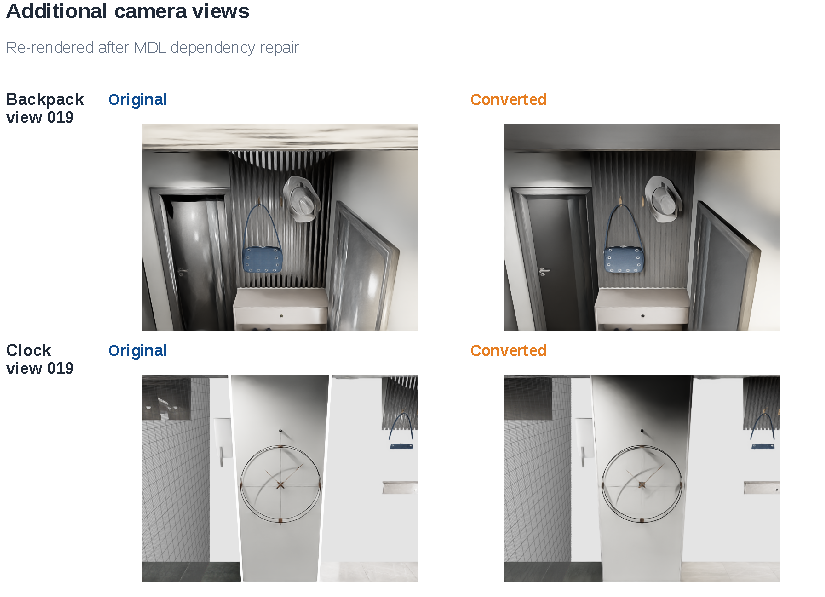
\includegraphics[width=\linewidth,height=.84\textheight,keepaspectratio]{appendix_grounding_diagnostics_02.pdf}
\caption{Additional target views after MDL dependency repair (1/2). Both material conditions are rerendered at the saved camera settings. These qualitative images are separate from the historical inference inputs and carry no prediction overlays.}
\label{fig:app-diagnostic1}
\end{figure}

\begin{figure}[p]
\centering
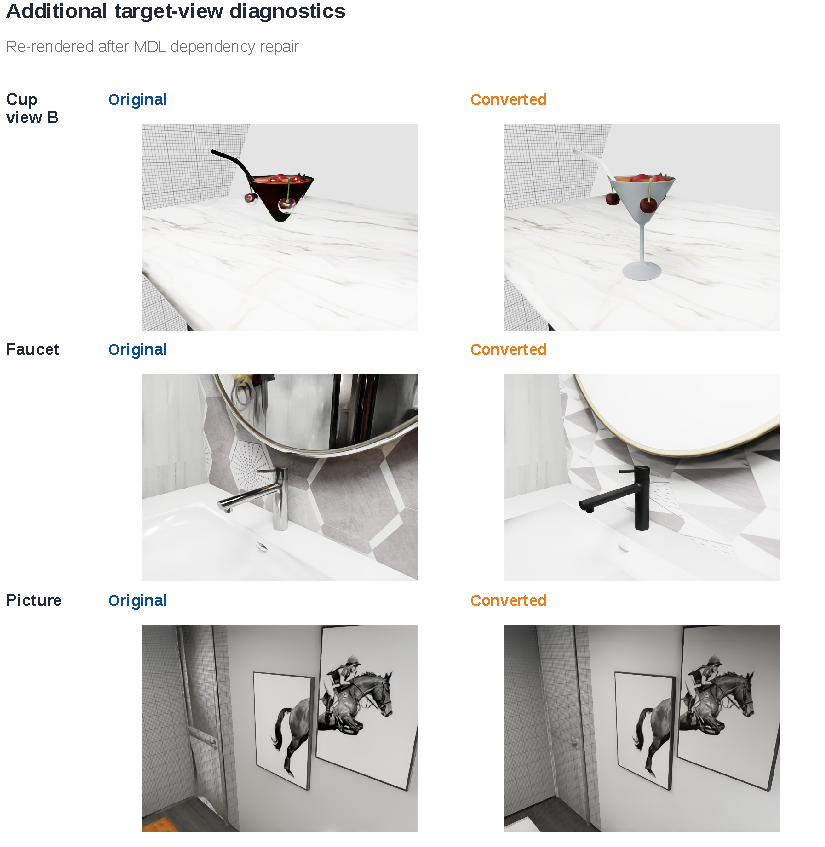
\includegraphics[width=\linewidth,height=.84\textheight,keepaspectratio]{appendix_grounding_diagnostics_01.pdf}
\caption{Additional target views after MDL dependency repair (2/2). Both material conditions are rerendered at the saved camera settings. These qualitative images are separate from the historical inference inputs and carry no prediction overlays.}
\label{fig:app-diagnostic2}
\end{figure}


\FloatBarrier
